\section{实证验证}
\label{sec:experiments}

我们评估使用 \sysname 训练 Transformer 模型的效果。
\begin{itemize}[itemsep=0.1pt,topsep=0pt,leftmargin=*]
  \item \textbf{注意力基准测试。}
  我们测量 \sysname 在不同序列长度下的运行时间，并与 PyTorch 标准实现、\sysnameone 以及 Triton 中的 \sysnameone 进行比较。
  结果确认：\sysname 相比 \sysnameone 快 1.7-3.0$\times$，相比 Triton 中的 \sysnameone 快 1.3-2.5$\times$，相比标准注意力实现快 3-10$\times$。
  在 A100 GPU 上，\sysname 最高可达 230 TFLOPs/s，即理论最大 TFLOPs/s 的 73\%。
  \item \textbf{端到端训练速度}
  当用于端到端训练 1.3B 与 2.7B 参数规模、序列长度为 2k 或 8k 的 GPT 风格模型时，\sysname 相比 \sysnameone 最高加速 1.3$\times$，相比不使用 \sysnameone 的基线最高加速 2.8$\times$。
  \sysname 在每张 A100 GPU 上最高达到 225 TFLOPs/s（模型 FLOPs 利用率 72\%）。
\end{itemize}

\subsection{注意力基准测试}
\label{subsec:benchmark_attn}

我们在 A100 80GB SXM4 GPU 上，在不同设置（不使用/使用因果掩码、head dimension 为 64 或 128）下测量不同注意力方法的运行时间。
结果见 \cref{fig:benchmark_attn_fwd_bwd}、\cref{fig:benchmark_attn_fwd}
与 \cref{fig:benchmark_attn_bwd}。
结果显示，\sysname 相比 \sysnameone 及 \texttt{xformers} 中的 \sysnameone（“cutlass” 实现）约快 2$\times$。
在前向传播中，\sysname 相比 Triton 中的 \sysnameone 约快 1.3-1.5$\times$；在反向传播中约快 2$\times$。
与 PyTorch 标准注意力实现相比，\sysname 最高可快 10$\times$。

基准设置如下：序列长度从 512、1k、...、16k 变化，并设置 batch size 使总 token 数为 16k。
隐藏维度设为 2048，head dimension 取 64 或 128（即分别为 32 个头或 16 个头）。
前向传播 FLOPs 按下式计算：
\begin{equation*}
  4 \cdot \text{seqlen}^2 \cdot \text{head dimension} \cdot \text{number of heads}.
\end{equation*}
使用因果掩码时，该值再除以 2，以反映大约仅有一半元素会被计算。
反向传播 FLOPs 则取前向 FLOPs 的 2.5 倍（由于前向有 2 次 matmul，反向因重计算有 5 次 matmul）。

\begin{figure}[ht]
  \centering
  \begin{subfigure}{.5\textwidth}
    \centering
    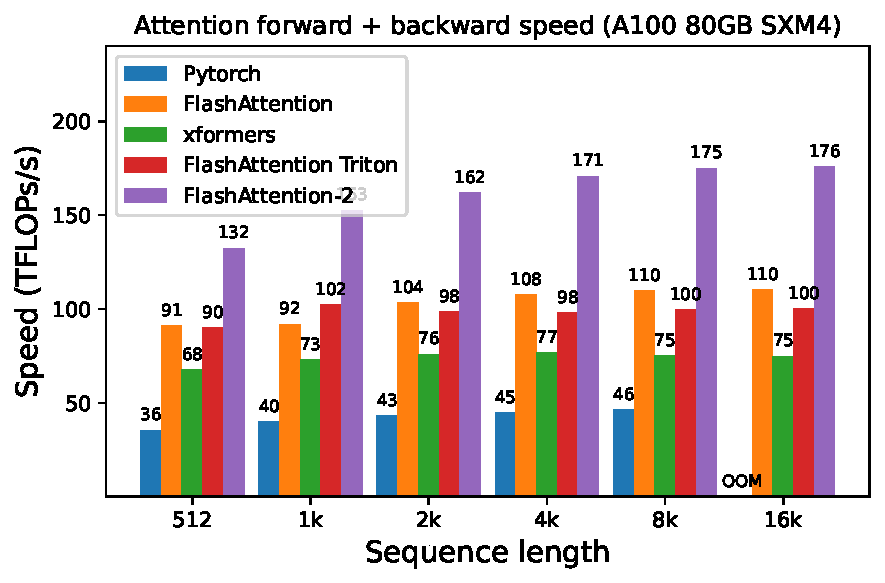
\includegraphics[width=.95\linewidth]{figs/flash2_causal_False_hdim_64_fwd_bwd_speed.pdf}
    \caption{无因果掩码，head dimension 64}
  \end{subfigure}%
  \begin{subfigure}{.5\textwidth}
    \centering
    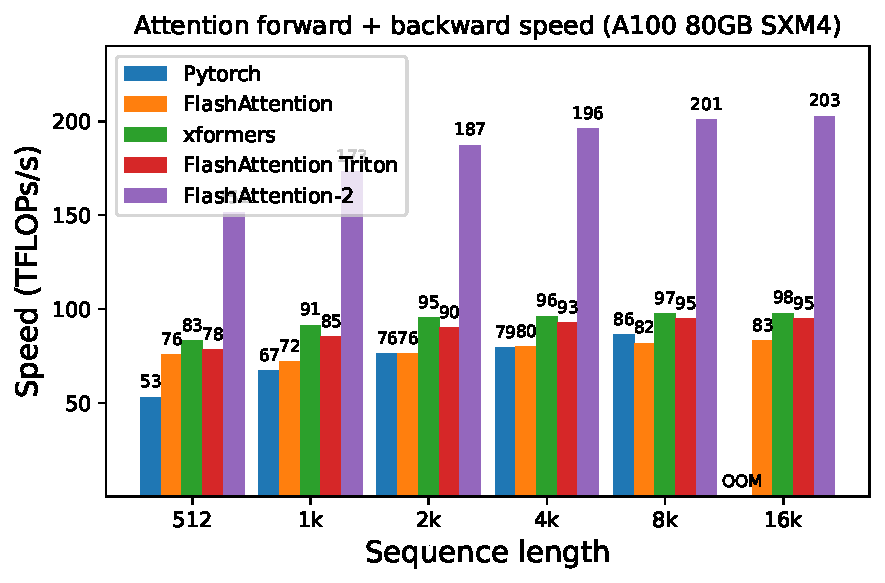
\includegraphics[width=.95\linewidth]{figs/flash2_causal_False_hdim_128_fwd_bwd_speed.pdf}
    \caption{无因果掩码，head dimension 128}
  \end{subfigure}
  \begin{subfigure}{.5\textwidth}
    \centering
    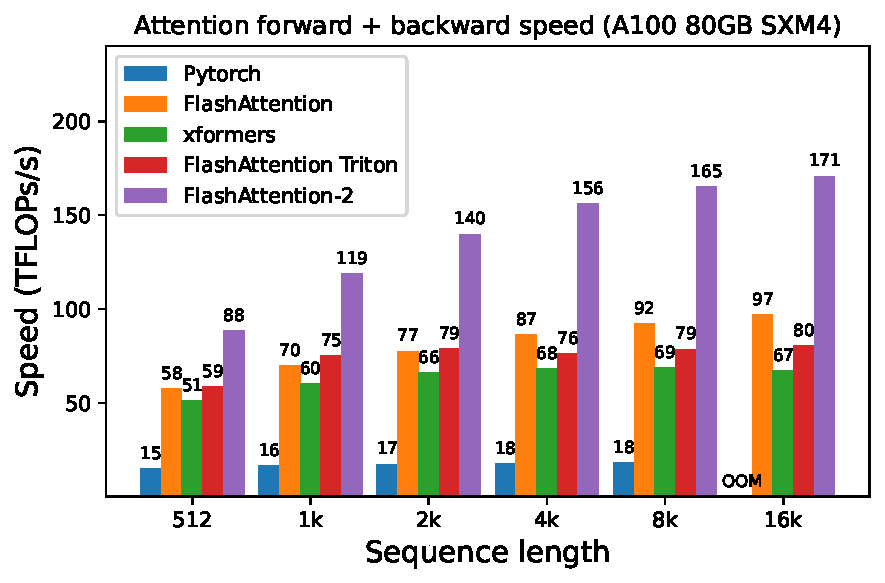
\includegraphics[width=.95\linewidth]{figs/flash2_causal_True_hdim_64_fwd_bwd_speed.pdf}
    \caption{有因果掩码，head dimension 64}
  \end{subfigure}%
  \begin{subfigure}{.5\textwidth}
    \centering
    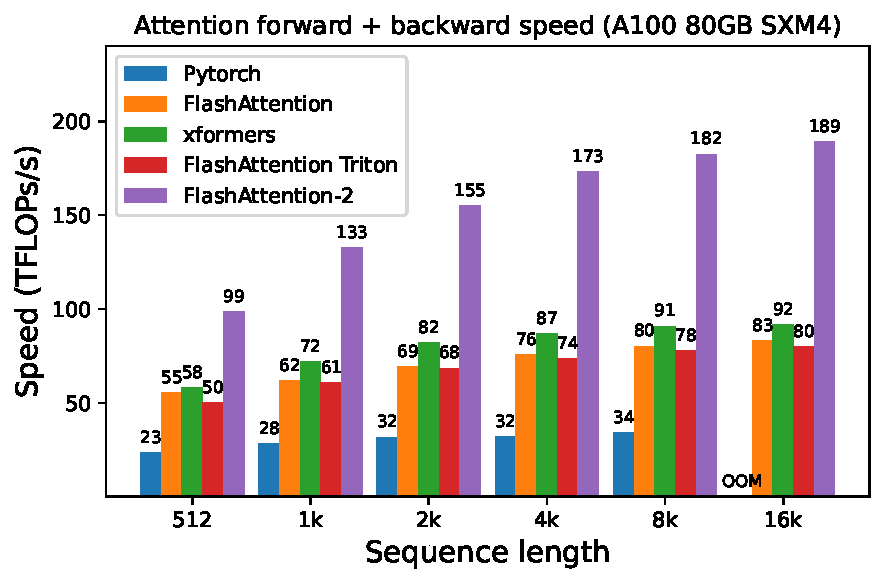
\includegraphics[width=.95\linewidth]{figs/flash2_causal_True_hdim_128_fwd_bwd_speed.pdf}
    \caption{有因果掩码，head dimension 128}
  \end{subfigure}
  \caption{A100 GPU 上注意力前向+反向速度}
  \label{fig:benchmark_attn_fwd_bwd}
\end{figure}

\begin{figure}[ht]
  \centering
  \begin{subfigure}{.5\textwidth}
    \centering
    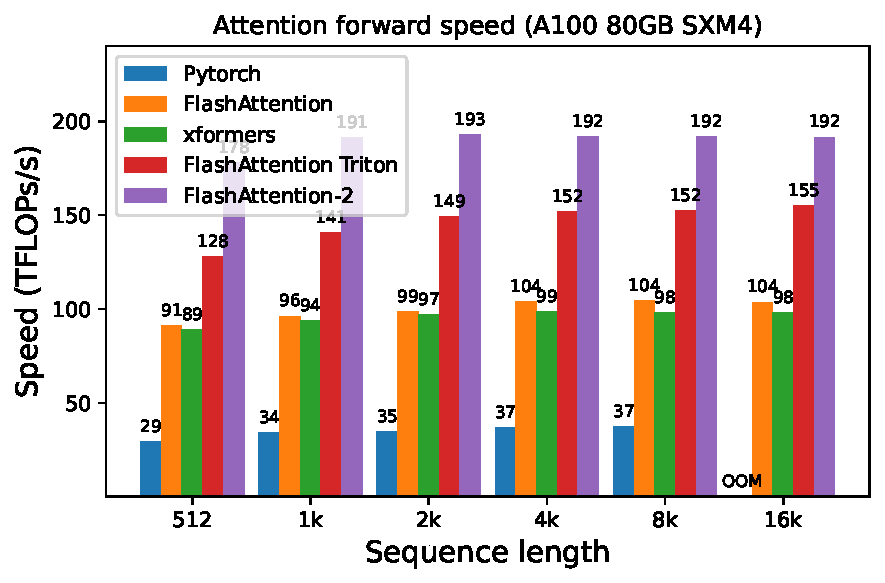
\includegraphics[width=.95\linewidth]{figs/flash2_causal_False_hdim_64_fwd_speed.pdf}
    \caption{无因果掩码，head dimension 64}
  \end{subfigure}%
  \begin{subfigure}{.5\textwidth}
    \centering
    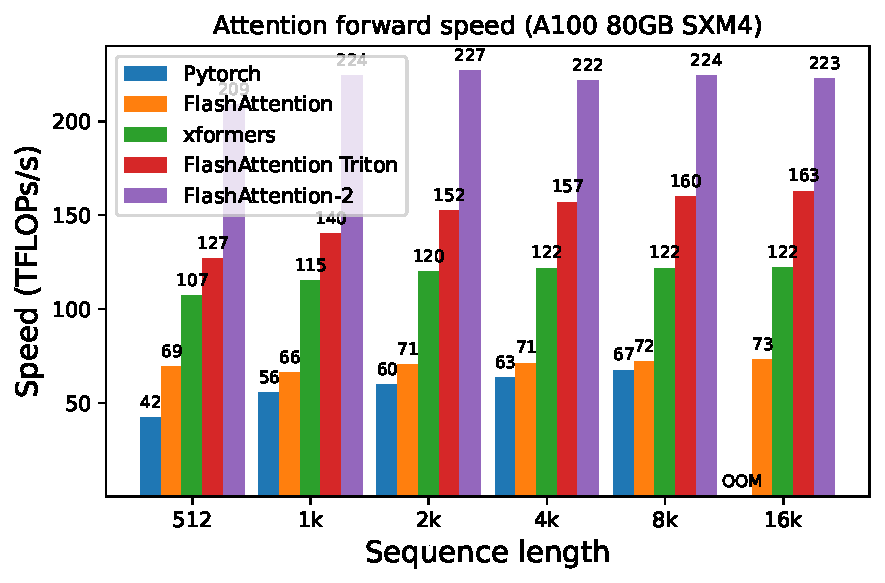
\includegraphics[width=.95\linewidth]{figs/flash2_causal_False_hdim_128_fwd_speed.pdf}
    \caption{无因果掩码，head dimension 128}
  \end{subfigure}
  \begin{subfigure}{.5\textwidth}
    \centering
    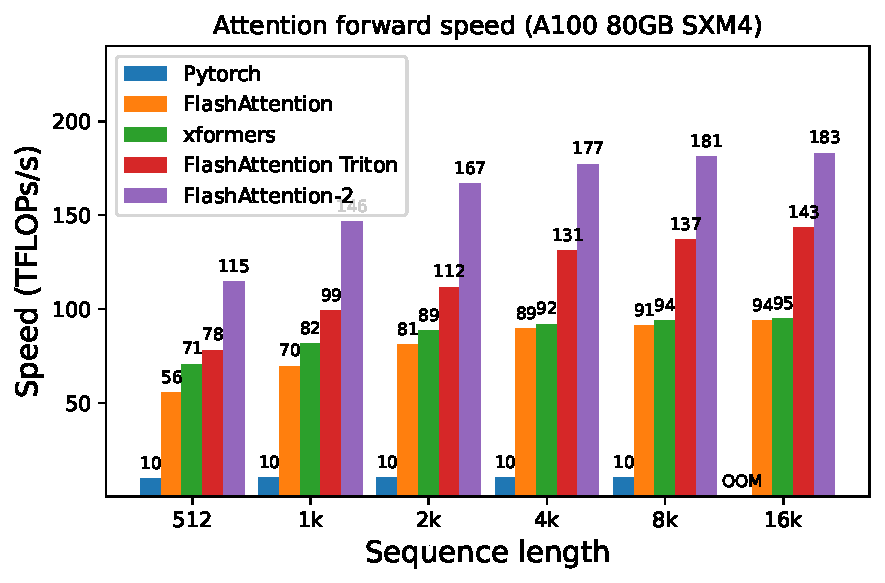
\includegraphics[width=.95\linewidth]{figs/flash2_causal_True_hdim_64_fwd_speed.pdf}
    \caption{有因果掩码，head dimension 64}
  \end{subfigure}%
  \begin{subfigure}{.5\textwidth}
    \centering
    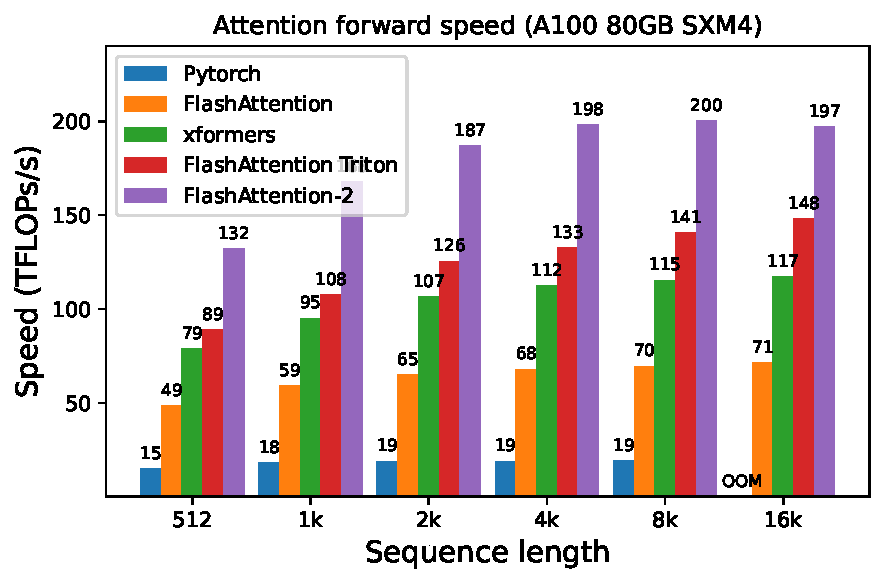
\includegraphics[width=.95\linewidth]{figs/flash2_causal_True_hdim_128_fwd_speed.pdf}
    \caption{有因果掩码，head dimension 128}
  \end{subfigure}
  \caption{A100 GPU 上注意力前向速度}
  \label{fig:benchmark_attn_fwd}
\end{figure}

\begin{figure}[ht]
  \centering
  \begin{subfigure}{.5\textwidth}
    \centering
    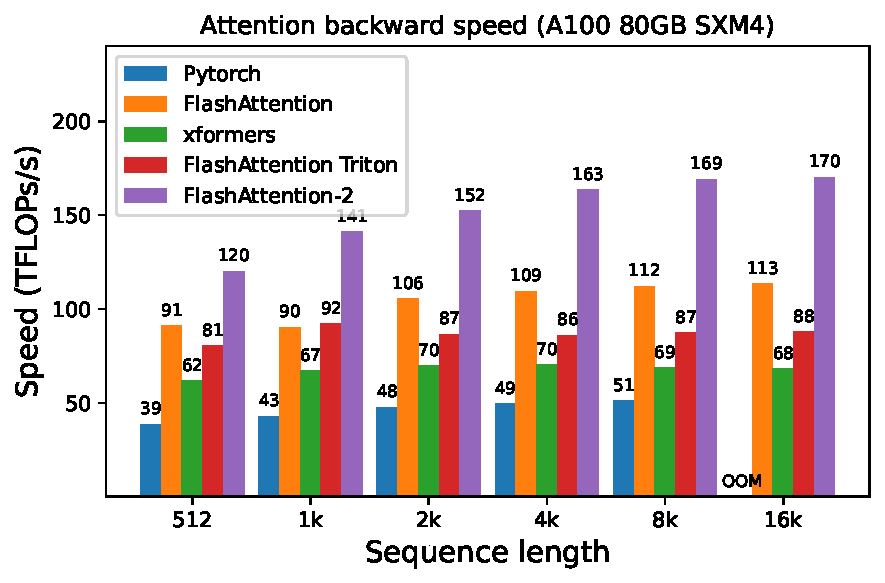
\includegraphics[width=.95\linewidth]{figs/flash2_causal_False_hdim_64_bwd_speed.pdf}
    \caption{无因果掩码，head dimension 64}
  \end{subfigure}%
  \begin{subfigure}{.5\textwidth}
    \centering
    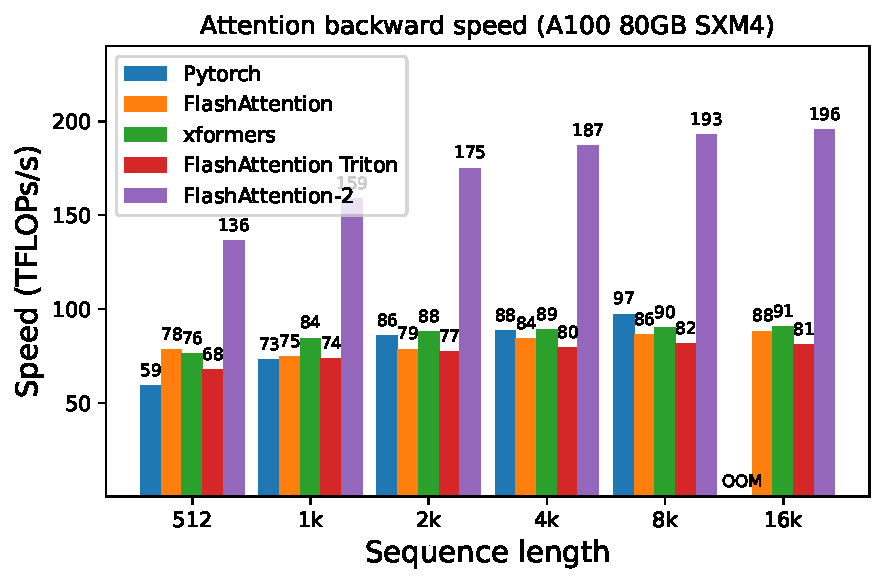
\includegraphics[width=.95\linewidth]{figs/flash2_causal_False_hdim_128_bwd_speed.pdf}
    \caption{无因果掩码，head dimension 128}
  \end{subfigure}
  \begin{subfigure}{.5\textwidth}
    \centering
    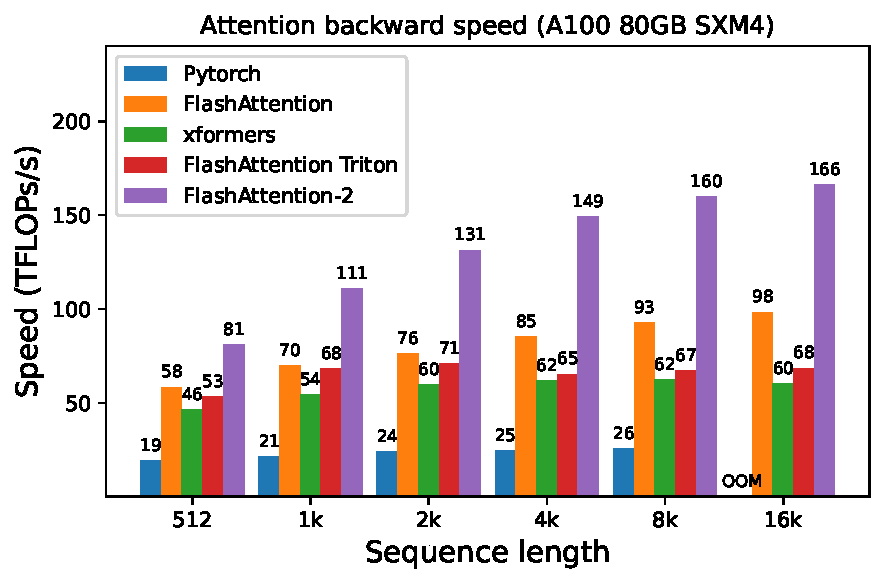
\includegraphics[width=.95\linewidth]{figs/flash2_causal_True_hdim_64_bwd_speed.pdf}
    \caption{有因果掩码，head dimension 64}
  \end{subfigure}%
  \begin{subfigure}{.5\textwidth}
    \centering
    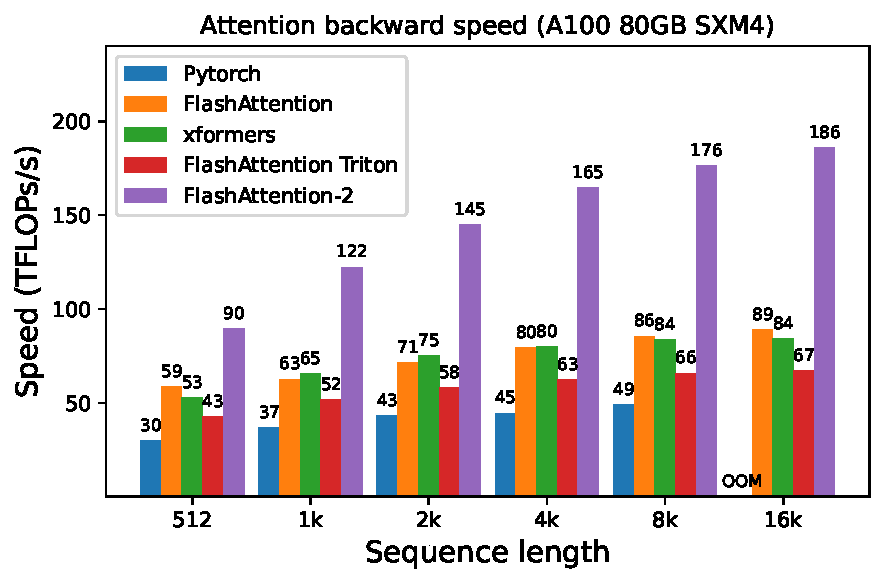
\includegraphics[width=.95\linewidth]{figs/flash2_causal_True_hdim_128_bwd_speed.pdf}
    \caption{有因果掩码，head dimension 128}
  \end{subfigure}
  \caption{A100 GPU 上注意力反向速度}
  \label{fig:benchmark_attn_bwd}
\end{figure}

仅将同一实现直接运行在 H100 GPU 上（未使用 TMA、第四代 Tensor Core 等新特性专用指令）时，我们可获得最高 335 TFLOPs/s（\cref{fig:benchmark_attn_fwd_bwd_h100}）。
我们预计若使用新指令，还能在 H100 上再获得 1.5x-2x 的加速，这留作未来工作。

\begin{figure}[ht]
  \centering
  \begin{subfigure}{.5\textwidth}
    \centering
    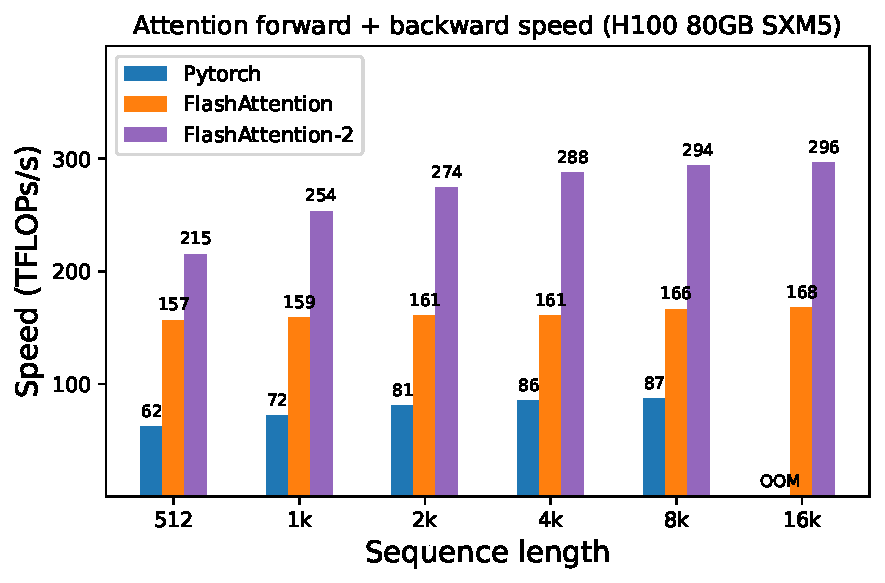
\includegraphics[width=.95\linewidth]{figs/flash2_h100_causal_False_hdim_64_fwd_bwd_speed.pdf}
    \caption{无因果掩码，head dimension 64}
  \end{subfigure}%
  \begin{subfigure}{.5\textwidth}
    \centering
    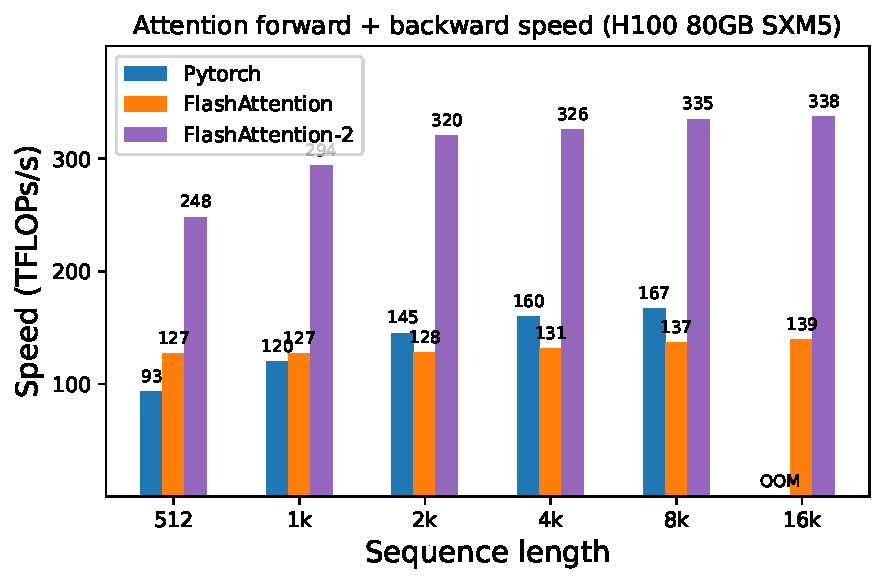
\includegraphics[width=.95\linewidth]{figs/flash2_h100_causal_False_hdim_128_fwd_bwd_speed.pdf}
    \caption{无因果掩码，head dimension 128}
  \end{subfigure}
  \begin{subfigure}{.5\textwidth}
    \centering
    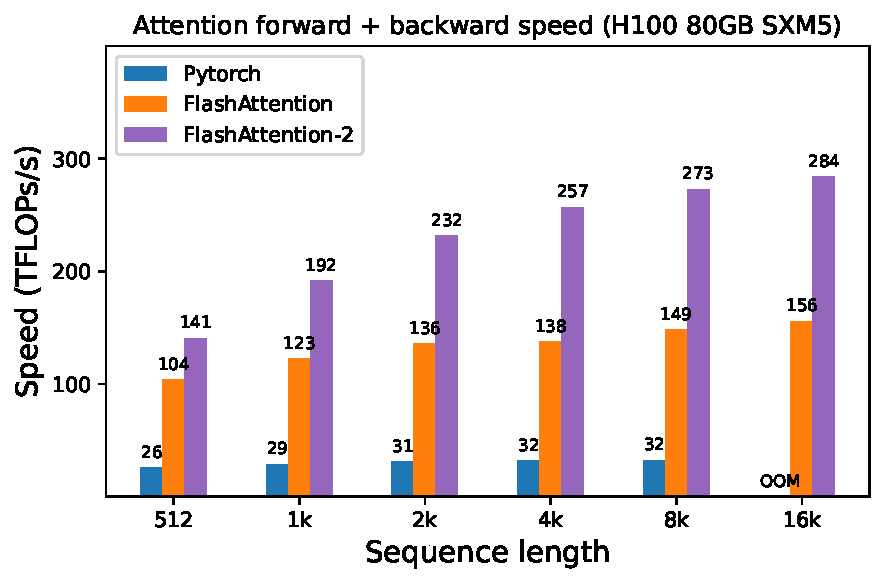
\includegraphics[width=.95\linewidth]{figs/flash2_h100_causal_True_hdim_64_fwd_bwd_speed.pdf}
    \caption{有因果掩码，head dimension 64}
  \end{subfigure}%
  \begin{subfigure}{.5\textwidth}
    \centering
    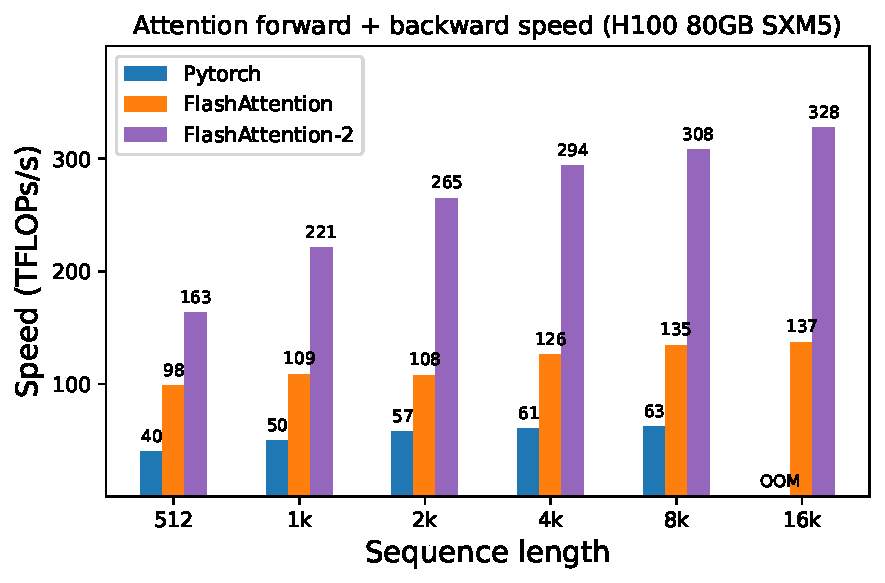
\includegraphics[width=.95\linewidth]{figs/flash2_h100_causal_True_hdim_128_fwd_bwd_speed.pdf}
    \caption{有因果掩码，head dimension 128}
  \end{subfigure}
  \caption{H100 GPU 上注意力前向+反向速度}
  \label{fig:benchmark_attn_fwd_bwd_h100}
\end{figure}

\subsection{端到端性能}
\label{subsec:end_to_end}

我们在 8$\times$A100 80GB SXM 上，测量参数规模为 1.3B 或 2.7B 的 GPT 风格模型训练吞吐。
如 \cref{table:end_to_end} 所示，\sysname 相比不使用 FlashAttention 的基线可达 2.8$\times$ 加速，相比 \sysnameone 可达 1.3$\times$ 加速，在每张 A100 GPU 上最高达到 225 TFLOPs/s。

需要说明的是，我们按下式计算 FLOPs，遵循 Megatron-LM~\citep{shoeybi2019megatron}（以及许多其他论文与库）：
\begin{equation*}
  6 \cdot \text{seqlen} \cdot \text{number of params} + 12 \cdot \text{number of
    layers} \cdot \text{hidden dim} \cdot \text{seqlen}^2.
\end{equation*}
第一项对应权重与输入相乘的 FLOPs，第二项对应注意力 FLOPs。
不过也可以认为第二项应减半，因为在因果掩码下大约只需计算一半注意力元素。
为保持一致性，我们采用文献中的公式（即不将注意力 FLOPs 再除以 2）。

\begin{table}[h!]
  \centering
  \caption{\label{table:end_to_end}8$\times$A100 GPU 上 GPT 风格模型训练速度（TFLOPs/s/GPU）。
    \sysname 最高达到 225 TFLOPs/s（模型 FLOPs 利用率 72\%）。
    对比基线为不使用 \sysnameone 的实现。
  }
    {
      \begin{tabular}{@{}c|ccc@{}}
        模型 & 不使用 \sysnameone & \sysnameone & \sysname \\ \hline
        GPT3-1.3B 2k 上下文 & 142 TFLOPs/s & 189 TFLOPs/s & 196 TFLOPs/s \\
        GPT3-1.3B 8k 上下文 & 72 TFLOPS/s & 170 TFLOPs/s & 220 TFLOPs/s \\
        GPT3-2.7B 2k 上下文 & 149 TFLOPs/s & 189 TFLOPs/s & 205 TFLOPs/s \\
        GPT3-2.7B 8k 上下文 & 80 TFLOPs/s & 175 TFLOPs/s & 225 TFLOPs/s \\
      \end{tabular}
    }
  \end{table}




%%% Local Variables:
%%% mode: latex
%%% TeX-master: "../flash2"
%%% End:
